%*********************第四章******************
\chapter{面向卷级神经网络前向过程的低延迟实现}
\section{引言}
随着卷级神经网络的应用越来越广,数据中心开始需要为用户提供神经网络前向计算过程的服务,而用户希望数据中心能够尽快响应,因此,在数据中心部署一个满足低延迟前向过程的神经网络具有重要的意义。特别是随着神经网络结构变得更深更复杂,处理的应用也由2D变为3D,所需的计算量不断地在增长,低延迟就更加重要了。而现有的数据中心一般都是拥有大量的计算资源,这为加速神经网络前向计算过程提供了硬件基础。针对数据中心大量的硬件计算资源,如何发挥计算资源的效能并且满足用户的低延迟需求变得尤为重要。对于神经网络的训练来说,用户不会有低延迟的需求,但对于神经网络的前向推测过程,用户是非常关注延迟的。神经网络的训练中采用的并行方法对于神经网络的前向推测过程就不适用了。神经网络的训练是以批处理的方式进行训练的,一次处理大量的输入,为了减少计算过程间的通信,一般采用数据并行的方式。而神经网络的前向推测过程一般需要立即处理用户提交的单个输入,虽然有多个计算设备,但却无法采用训练中数据并行的方式进行加速,而需采用模型并行的方法才能达到低延迟的目标。模型并行是将模型参数分割在多个计算设备,这也可以解决模型参数过大在单个设备存储不足的问题,此外,神经网络每一层网络的计算都是由多个计算设备一起完成的,在每一层计算结束之后,各个计算设备间需要通信进行数据交换。

本章的目的主要是在数据中心环境下解决神经网络前向推测过程的低延迟问题。其中涉及到在多个计算设备上并行的问题,本章主要介绍如何采用模型并行的技术来对神经网络进行加速计算,并对模型并行中涉及到的通信问题,采用CUDA-Aware MPI技术使得GPU间通信更加高效,并且对多个计算设备间的通信模式进行了优化,使得通信代价不会随着计算设备的增多而增大。最后采用计算与通信进行重叠计算的技术进一步提升性能,这需要对模型并行进行流水化处理。

本章内容安排如下:第二节将介绍针对神经网络加速的相关研究,有针对算法的改进进行加速的方法,也有面向多设备采用数据并行和模型并行方法的相关研究;第三节主要介绍了关于数据并行、模型并行以及GPU间高效通信的CUDA-Aware MPI接口;第四节将主要介绍模型并行的流水化,具体包括模型并行的流水化实现,优化的通信模式设计以及计算与通信重叠的执行;最后一节将介绍实验部分,主要是2D以及3D卷级层的模型并行性能的测试。

\section{相关研究}
\label{relatedwork}
本章处理的神经网络为卷积神经网络,卷积神经网络的计算集中在卷积层,下面主要介绍针对卷积计算的加速的相关研究。首先是卷积算法的改进,Mathieu等人采用傅立叶变换的方法\ref{}实现卷积计算,这种方法在卷积核大小比较大的时候优势明显,因为卷积核大小在一定范围内变化时,比如3~16,傅立叶方法所需的计算量不会随着卷积核大小变化而变化,而对于传统卷积方法来说,卷积核越大意味着卷积所需的计算量越大,因此,在卷积核比较大时,选择傅立叶方法在计算量方面有明显的优势,而傅立叶方法存在的问题就是所需的存储开销大,这成为限制傅立叶方法普遍使用的重要障碍。Lavin等人\ref{}将一个称为Winograd的算法应用在2D卷积计算中,并且在GPU平台上高效地实现了Winograd算法。Winograd算法是传统卷积计算方法与傅立叶方法的一种折中,即在保持存储开销不变的条件下降低计算量,最后的实验结果也表明,他们在GPU上的高效实现最后性能超过目前最快的cuDNN库。Winograd算法也非常适合在硬件加速平台上实现,Aydonat等人\ref{}就将Winograd算法在FPGA平台上采用高级语言进行了实现。不过这些Winograd算法的实现目前还只针对2D卷积网络。

另一种加速卷积网络计算的思路是将其中的浮点计算转化为代价更小的计算类型。比如将32位的浮点运算转化为16位浮点或者8位浮点运算,而这基本不会影响结果的精度。有些工作比如\ref{}、\ref{}甚至将卷积计算的输入和模型参数转化为4位或者2位。而Rastegari等人\ref{}提出了一个XNOR网络,这个网络的输入和模型参数都是用1位来表示,而它们之间的计算则转化为异或计算,这些方法不但简化了计算而且还节省了存储开销,但存在精度下降的问题。

以上研究都还集中在单设备上对神经网络进行加速。Alex等人\ref{}针对神经网络的训练提出了一个混合并行的方法,这个方法主要是用在多GPU设备上,他们根据神经网络的特点,比如卷积层计算量比较大,模型参数比较少,因此,针对卷积神经网络的卷积层使用数据并行的方式,而对于卷积神经网络的全连接层,由于全连接层参数规模较大,采用模型并行的方式,这种混合并行的方式可以有效减少数据通信。在对神经网络的训练中,Awan等人专门提出了S-Caffe\ref{},S-Caffe的采用了计算与通信重叠的技术对多GPU间的通信进行了优化。而本章工作提出了流水化的模型并行方式对神经网络的前向计算过程进行加速,并且对模型并行中的通信进行了优化。

\section{数据并行、模型并行以及CUDA-Aware MPI}
本节将介绍在神经网络中常用的两种并行方式,数据并行和模型并行,此外,本章还将介绍在多GPU件高效通信使用的CUDA-Aware MPI 进行介绍。

\subsection{数据并行与模型并行}
多GPU环境下,存在两种并行方式对卷积神经网络进行加速,即数据并行和模型并行。在数据并行中,所有的工作线程计算过程一样,每个工作线程独立地处理不同的输入,因此数据并行方式可以有效地增加处理输入的吞吐率。对于模型并行来说,每一层卷积德模型参数都被分割到不同的计算设备中,然后每一个工作线程都只负责部分结果的计算,计算结束后,所有工作线程之间需要交换计算的结果,计算设备越多,意味着所需的通信也越多。但由于所有的计算设备同时处理卷积神经网络的每一层计算,所以,模型并行可以显著降低卷积神经网络前向推测过程的延迟,并且针对大型的卷积神经网络,由于模型参数分布在不同的计算设备中,可以解决单个设备无法存储所有模型参数的问题。图\ref{dataAndModelParallel}为数据并行与模型并行的示意图。


\begin{figure*}[tbh]%\small
\centering
%\resizebox{0.5\textwidth}{!}{
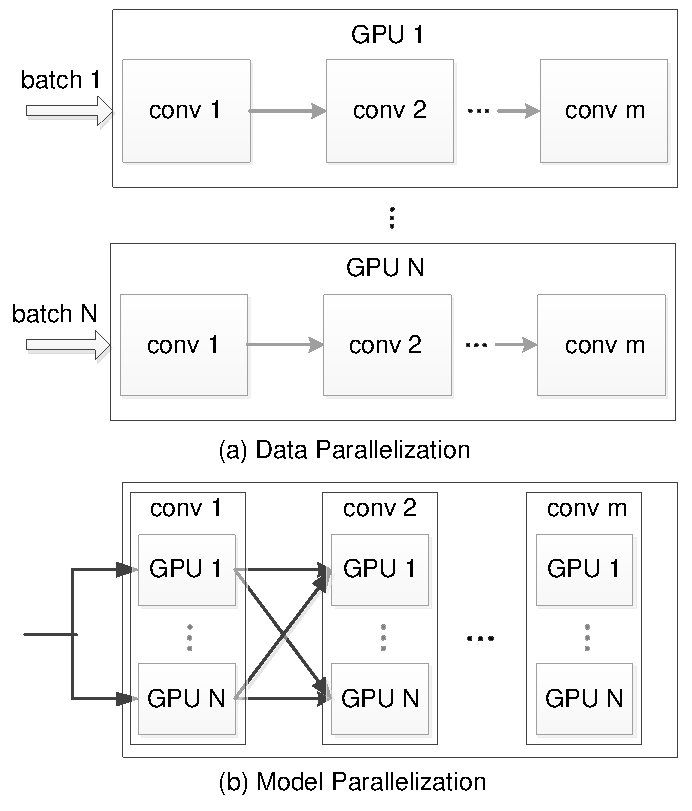
\includegraphics[width=12cm]{figs/dataAndModelParall.pdf}
%}
\caption{数据并行与模型并行.}
\label{dataAndModelParallel}
\end{figure*}

\subsection{CUDA-Aware MPI}
英伟达公司提供的GPUDirect技术使得读写GPU设备存储和主机存储变得更加直接和高效,可以减少很多不必要的数据拷贝,显著地降低CPU开销以及减少访存延迟。基于GPUDirect技术,英伟达公司在2011年更是提供了点到点的GPUDirect支持,使得处于同一PCIE连接下的GPU设备间可以相互访问各自的显存。而后面提出的GPUDirect DMA技术则解决了CPU主存与GPU显存间高效数据传输的问题。

对于单节点内多GPU的异构平台,可以采用多线程的方式对各个GPU进行控制,GPU之间的通信将分两步完成,比如需要将GPU A的显存数据传输到GPU B显存中,控制GPU A的线程首先将数据从GPU A拷贝到CPU 主存中,然后控制GPU B的线程将数据从CPU的主存拷贝到GPU B的显存中。线程这种显式控制数据传输的方式虽然很直接,但程序的移植性不够好,当异构节点中GPU数量变化时,程序就需要改写。我们将介绍我们所采用的编程方式即MPI编程,MPI编程最开始运用在多节点环境下,节点间是对等的关系,针对单个节点内多GPU情形下,也同样可以创建多个MPI进程,每个MPI进程控制一个GPU,GPU间通信通过MPI间通信实现。而自从Nvidia对统一虚拟地址(UVA)以及GPUDirect技术的支持,通过MPI编程控制GPU间通信变得更加简单和高效。基于UVA和GPUDirect技术,无论是现在的OpenMPI还是MVAPICH2都支持CUDA-Aware MPI原语,所谓的CUDA-Aware MPI原语是能识别CPU主存和GPU显存从而自动完成底层硬件通信通路的最优选择,所以CUDA-Aware MPI不但编程简单,而且也是通信最高效的一种编程方法。图为CUDA-Aware MPI的示意图。CUDA-Aware MPI还支持飞阻塞通信,这为计算与通信重叠的使用提供基础。

\section{模型并行优化}
这一节将介绍模型并行的简单实现以及模型并行的流水化实现。模型并行的简单实现只是将原来在单个GPU执行的卷积运算通过模型并行在多个GPU上实现,简单的模型并行实现分成两阶段,第一阶段是计算,第二阶段是通信;模型并行的流水化实现就是将计算分割成很多小的计算任务,在每个小的计算任务完成后进行一次通信,计算和通信交替地进行,第i次计算任务后的通信可以与第i+1次计算任务并行的执行,这就是模型并行的流水化实现。流水化的执行可以对通信进行隐藏,降低通信开销。本章还会介绍一种优化的通信模式,这种通信模式不会随着计算设备的增多而增加通信的代价。

\subsection{模型并行的简单实现}
前面已经介绍了关于模型并行的概念,我们主要将模型并行应用到卷积神经网络的卷积层,本节将介绍模型并行的简单实现。

单计算设备的卷积层实现不涉及通信过程,只包含计算过程,卷积计算的实现可以采用目前流行的库,比如cublas或者cuDNN(针对GPU平台)。针对多计算设备的模型并行实现,包含计算和通信两个过程,



基于GPUDirect技术的模型并行实现如算法\ref{}所示。

下面从理论上分析单设备

\subsection{模型并行的流水化实现}

\subsection{优化的通信模式设计}


%\subsection{计算与通信的重叠执行}

\section{实验评测与分析}

\subsection{实验设置}

\subsection{2D卷级层模型并行实现性能}

\subsection{3D卷级层模型并行实现性能}


\section{小结}
面对跟踪器日益复杂的结构和不断增加的计算负载,高性能的跟踪算法实现变得十分必要。
